\chapter{Baggrund}

Responsum K/S er en virksomhed der besvarer andre virksomheders opkald, som en ekstern reception. Det vil sige at hvis f.eks. den lokale skorstensfejer har problemer med at tage telefonen når han sidder på folks tage, så kan han få en aftale med Responsum K/S, så han omstiller alle sine opkald dem, hvor der sidder receptionister klar til at tage imod hans kunder når de ringer. Receptionisterne kan så se på baggrund af hans kalender eller hvad der ellers er aftalt om de skal prøve at ringe skorstensfejeren op, eller tage imod en besked så skorstensfejeren ikke mister sine kunder på at han ikke kan svare sin telefon.

For at kunne dette gør de brug af telefonanlæg, databaser og PC baserede klienter. Deres nuværende system er udviklet tilbage i 90'erne og består for en stor del af komponenter der ikke længere udvikles på, og derfor efterhånden slæber rundt på en del fejl og mangler. Som følge heraf gik Adaheads K/S igang med at udvikle et fremtidssikret open source system baseret på GPL licensen for at sikre, at koden altid er tilgængelig for systemets brugere.

Responsum K/S har behov for at kunne lave kaldplaner til at modtage og dirigere opkald til henholdsvis receptionister eller automatiske systemer som IVR menuer og telefonsvarer. Der skal knyttes information til alle indgående opkald, sådan at receptionister og systemer kan håndtere dem korrekt. For at kunne oprette og vedligholde kaldplaner og virksomhedsinformation skal der være administrative værktøjer til rådighed.

\section{AdaHeads produkt}
AdaHeads' produkt bestod af systemerne der kan ses på firgur~\ref{fig:adaheadssystembefore}. Der vil være en gennemgang i kapitel~\ref{sec:adminSystemoversigt} af hvilke nye dele der blev tilføjet.
\begin{figure}[ht!]
\centering
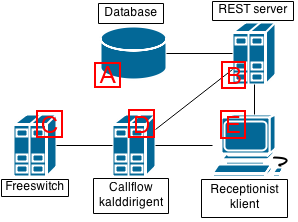
\includegraphics[scale=0.5]{images/system_before_admin.png}
\caption{En oversigt over Adaheads system.}
\label{fig:adaheadssystembefore}
\end{figure}
\begin{enumerate}
	\item[A.]{Relationel database}
	\item[B.]{REST intefaces, fordelt på flere HTTP servere}
	\item[C.]{Freeswitch PBX til håndtering af opkald} 
	\item[D.]{CallFlow kald dirigenten håndterer kaldrelateret kommunikation mellem Freeswitch og resten af systemet}
	\item[E.]{Browser baseret klient til receptionister}
\end{enumerate}
